\documentclass{beamer}
%\documentclass[notes=only]{beamer}

\usepackage[utf8]{inputenc}
\usepackage{listings}
\usepackage{ulem}
\usepackage{hyperref}
\usepackage{amsmath}

\lstdefinestyle{customcbig}{
  belowcaptionskip=1\baselineskip,
  breaklines=true,
%  frame=L,
  xleftmargin=\parindent,
  language=C,
  showstringspaces=false,
  basicstyle=\small\ttfamily,
  keywordstyle=\bfseries\color{green!40!black},
  commentstyle=\itshape\color{purple!40!black},
  identifierstyle=\color{blue},
  stringstyle=\color{orange},
}

\lstdefinestyle{customc}{
  belowcaptionskip=1\baselineskip,
  breaklines=true,
%  frame=L,
  xleftmargin=\parindent,
  language=C,
  showstringspaces=false,
  basicstyle=\scriptsize\ttfamily,
  keywordstyle=\bfseries\color{green!40!black},
  commentstyle=\itshape\color{purple!40!black},
  identifierstyle=\color{blue},
  stringstyle=\color{orange},
}

\lstdefinestyle{customctiny}{
  belowcaptionskip=1\baselineskip,
  breaklines=true,
%  frame=L,
  xleftmargin=\parindent,
  language=C,
  showstringspaces=false,
  basicstyle=\tiny\ttfamily,
  keywordstyle=\bfseries\color{green!40!black},
  commentstyle=\itshape\color{purple!40!black},
  identifierstyle=\color{blue},
  stringstyle=\color{orange},
}
 
\usetheme{Dresden}

\title[SOFTENG 370 Tutorial 7 (2019)] %optional
{Exam Revision}
  
\author{Edward Zhang}
 
% \institute[UoA] % (optional)
% {
%   Department of ECSE\\
%   The University of Auckland
% }
 
\date[October 2019] % (optional)
{SOFTENG 370 T7}

\begin{document}
\frame{\titlepage}
\begin{frame}
  \frametitle{Exam Info}
  Your exam will be short answer, not MCQ. That means the exam from 2012 - 2017 aren't very useful. 2018 had a different lecturer for the first $\frac{1}{2}$ so it's not super helpful either.\\
\end{frame}
\section{Adapted MCQs}
\begin{frame}
  \frametitle{Instructions which query the running state of a processor (i.e. kernel or user mode) make virtualization difficult. Why?}
  \pause
  Consider trap and emulate virtualization, where we expect privileged instructions from the guest to throw exceptions that the VMM can trap.
  \pause
  \begin{block}{Answer}
    An instruction running in the kernel of a guest operating system would report that it was running in user mode.
  \end{block}
\end{frame}
\begin{frame}
  \frametitle{In order to allow safe multiprogramming what hardware advances needed to be made?}
  \pause
  Key word: Safe. How can we keep tasks isolated from each other (recall we need two things for this, one alone won't work), and how do we allow for effective time sharing?
  \pause
  \begin{block}{Answer}
    Hardware memory protection, interrupt processing, privileged instructions.
  \end{block}
\end{frame}
\begin{frame}
  \frametitle{Which of the following statements about files is FALSE?}
  \begin{itemize}
    \item<alert@2> All Unix files are stored on secondary storage.
    \item With sparse files it is possible to have the size of a file larger than the device the file is stored on.
    \item Executable files have different structures specific to their particular operating systems.
    \item Moving a file does not necessarily mean that all of the data needs to be copied then the original file deleted.
  \end{itemize}
  \pause
  \begin{block}{Explanation}
    Counterexample: \texttt{tmpfs}
  \end{block}
\end{frame}
\begin{frame}
  \frametitle{Which of the following statements about NFS is TRUE?}
  \begin{itemize}
    \item NFS only works in a homogeneous environment with all clients and servers running the same operating system.
    \item Servers in NFS are dedicated to acting as file servers and cannot be used for general operations.
    \item<alert@2> NFS mounts remote directories in a similar way to the method Unix mounts drives in the directory tree.
    \item Remote file directories in NFS can only be mounted when a machine is booted.
  \end{itemize}
  \pause
  \begin{block}{Explanation}
    Recall that NFS maintains a mapping of directories to remote servers that they're mounted on.
  \end{block}
\end{frame}
\begin{frame}
  \frametitle{Which of the following is NOT usually considered a requirement in a language used for operating system implementation?}
  \begin{itemize}
    \item It is easy to produce fast and efficient code with the language.
    \item The language allows access to memory locations.
    \item The language is compiled.
    \item<alert@2> The language is dynamic and weakly typed
  \end{itemize}
  \pause
  \begin{block}{Explanation}
    Counterexample: Almost every language used to write an OS isn't dynamically typed.
  \end{block}
\end{frame}
\begin{frame}
  \frametitle{Which of the following best describes the Confused Deputy problem?}
  \begin{itemize}
    \item A program with privileges is tricked into giving those privileges to another program.
    \item<alert@2> A program with privileges is tricked into misusing its authority.
    \item A program with privileges gets so many requests that it loses track of which request came from which source.
    \item A program with privileges mistakenly prevents access to a resource which should be available. 
  \end{itemize}
  \pause
  \begin{block}{Example}
    You ask the deputy (say \texttt{passwd}) to do something for you that it shouldn't (change someone else's password) and it obliges.
  \end{block}
\end{frame}
\begin{frame}
  \frametitle{Order these file block allocation techniques from most efficient to least efficient for random access to file information.}
  “Efficient” for this task relates to the number of different block reads necessary to access the file information
  \begin{itemize}
    \item Single-level Indexed allocation
    \item Contiguous allocation
    \item Multi-level Indexed allocation
    \item Linked Allocation
  \end{itemize}
  \pause
  \begin{block}{Answer}
    Contiguous allocation (trivial), single-level indexed allocation (access only one index block), multi-level indexed allocation (access multiple index block), linked allocation (linked-list like).
  \end{block}
\end{frame}
\begin{frame}
  \frametitle{Describe locality of reference and why it is important?}
  Consider in the context of virtual memory and also filesystems, especially network ones.
  \pause
  \begin{block}{Answer}
    Many memory or file accesses in a small period of time are close together. This is important for the efficiency of virtual memory (loading in memory from swap), read-ahead in file data and in distributed file systems.
  \end{block}
\end{frame}
\begin{frame}
  \frametitle{Which of the following statements best describes what is being depicted in the figure?}
  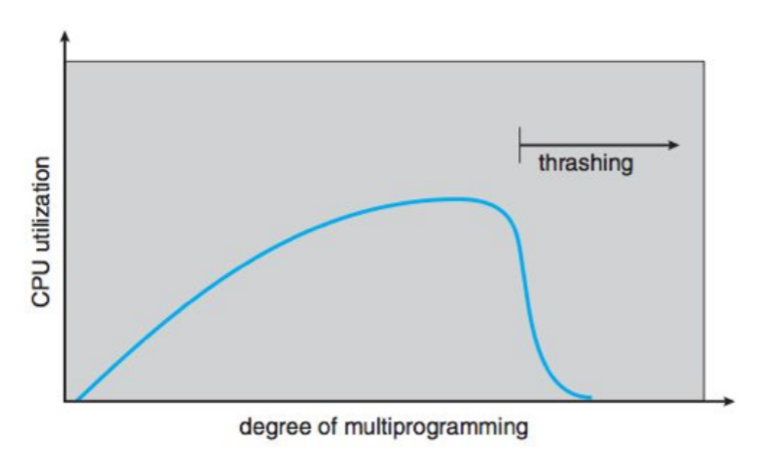
\includegraphics[width=\textwidth,height=0.8\textheight,keepaspectratio]{images/thrashing.png}
\end{frame}
\begin{frame}
  \frametitle{Cont.}
  \begin{itemize}
    \item Increasing the amount of multiprogramming will increase the CPU utilization until the file system can no longer deal with the read/write requests and the hard drives crash.
    \item<alert@2> Running too many processes can cause thrashing in the virtual memory system which means that very little work can get done by any process.
    \item Increasing CPU utilization allows the number of processes to increase until a limit is reached and most of the processes finish.
    \item When thrashing begins the amount of free CPU time goes up dramatically this means that more processes can now be scheduled.
    \item All of the above.
  \end{itemize}
\end{frame}
\begin{frame}
  \frametitle{Which of the following is NOT a way to prevent deadlock?}
  \begin{itemize}
    \item Only allow groups of resources to be allocated at once. If another group needs to be allocated first release the current group of resources.
    \item Only allow resources to be collected in a set order.
    \item<alert@2> Use time stamps to determine the order of requests and give the resource to the one which has been waiting the longest.
    \item Use the Banker’s algorithm to control resource requests.
    \item Allocate all resources a process needs as the program begins.
  \end{itemize}
  \pause
  \begin{block}{Explanation}
    Different programs may need resources with different delays, thus this can still result in deadlock.
  \end{block}
\end{frame}
\section{Selected 2018 Exam Questions}
\begin{frame}[fragile]
  \frametitle{Question 5}
  Here is pseudo code for simple lock and unlock operations. The variable "locked" is true if the lock is currently being held and false otherwise.
  \begin{lstlisting}[style=customc]
    lock:
      while locked
        sleep 10 msec
      locked = true

    unlock:
      locked = false
  \end{lstlisting}
  \begin{itemize}
    \item Is this lock a busy wait?
    \item Could this lock provide mutual exclusion to a critical section of code?
  \end{itemize}
\end{frame}
\begin{frame}
  \frametitle{Question 5 Answers}
  \begin{block}{Is this lock a busy wait?}
    No, since it sleeps most of the time. Bit confusing due to the loop. In a busy wait, the process is running continuously checking the lock variable
  \end{block}
  \begin{block}{Could this lock provide mutex?}
    No. If it's unlocked and two processess call lock at the same time, both would see the locked value as false and set it as true. The check and set isn't atomic.
  \end{block}
\end{frame}
\begin{frame}
  \frametitle{Question 7a}
  How much memory is used by a full page table on a system with a virtual address space of 32-bits and pages of size 4Kbytes, and where each page table entry is 8 bytes long?
  \pause
  \begin{block}{Calculation}
    \begin{enumerate}
      \item Virtual address space contains $2^{32}$ bytes
      \pause
      \item Divide by a page size of 4KB ($2^{12}$ bytes), gives us the number of page table entries
      \pause
      \item Multiply by the size of each entry, 8 bytes ($2^3$ bytes)
      \pause
      \item $\frac{2^{32}}{2^{12}}\times 2^3 = 2^{23}$ bytes, or 8MB
    \end{enumerate}
  \end{block}
\end{frame}
\begin{frame}
  \frametitle{Question 8a/b}
  Briefly discuss one advantage and disadvantage of filesystems in userspace.
  \pause
  \begin{block}{Answer}
    \begin{enumerate}
      \item The file system is isolated from the kernel. The system can then be extended and modified without heightened privileges. This provides flexibility to ordinary programmers and increased protection of
      the system.
      \item File system calls may transition from user to kernel space multiple times, making the system slightly less efficient than a kernel space file system.
    \end{enumerate}
  \end{block}
\end{frame}
\begin{frame}
  \frametitle{Question 9b}
  One protection against the Meltdown exploit that has been implemented in operating systems is kernel page-table isolation (KPTI). Explain what kernel page-table isolation is.
  \pause
  \begin{block}{Answer}
    Separate page tables are kept for a process when it is running in kernel and user mode. The user mode page tables do not have most of the kernel pages mapped into them.
  \end{block}
\end{frame}
\begin{frame}
  \frametitle{Question 9c/d}
  What effect could KPTI have on efficiency, and how does it prevent Meltdown?
  \pause
  \begin{block}{Efficiency}
    Anything that switches to kernel mode, like syscalls, requires a new page table to be loaded. This will also likely flush the TLB.
  \end{block}
  \pause
  \begin{block}{Preventing Meltdown}
    Meltdown's timing attack relies on attempts to access values in kernel address space (even if these are eventually rejected by a privledge check). However, with KPTI, those addresses are not accessible in the current address space, so the attempt cannot be made.
  \end{block}
\end{frame}
\section{Selected 2011 Exam Questions}
\begin{frame}
  \frametitle{Question 1a}
  Use the Dining Philosophers' problem to demonstrate deadlock
  \pause
  \begin{block}{Answer}
    We have a circle of philosophers with a chopstick (originally fork, but that doesn't really make sense) shared between each adjacent pair of philosophers. The philosophers have to pick both chopsticks (to the left and to the right of them) and each of them can pick up one chopstick. In this way every philosopher is also waiting for a chopstick and they are all deadlocked.
  \end{block}
\end{frame}
\begin{frame}
  \frametitle{Question 2a}
  Explain the difference between soft links and hard links to a file
  \pause
  \begin{block}{Answer}
    \begin{itemize}
      \item A soft link is a special type of file (usually a text file) which contains a pointer to the original file (usually just its full or relative pathname). The file system uses the soft link to find the real file.
      \item A hard link is another name for the file. The actual file information is stored somewhere else, such as the Master File Table or the inode table, and all hard links refer to that information. The file information must hold a count of how many hard links there are to the file.
    \end{itemize}
  \end{block}
  What are soft links usually called in Linux and how does one create them?
  \pause
  A: Symbolic links. Created using \texttt{ln -s}
\end{frame}
\begin{frame}
  \frametitle{Question 3a}
  What is location transparency and why is it a desirable property for a distributed file system?
  \pause
  \begin{block}{Answer}
    Location transparency means that the location of a resource or file is not related to its name. It is desirable because users and programs should be able to locate files without having to know what server they are on. It also makes it possible to migrate the resource to another location without breaking programs which refer to it.
  \end{block}
\end{frame}
\begin{frame}
  \frametitle{Question 2d}
  NTFS stores the information about the location of file data on a disk using extents. Describe what “extents” are and explain how a particular cluster or block in a file can be located on disk from the information in the list of extents.
  \pause
  \begin{block}{Answer}
    An extent consists of a starting cluster number and a number of contiguous clusters. To find a particular cluster we traverse the list of extents, adding the size of the extents as we go. When the total first exceeds the particular cluster number we are searching for we have found the extent holding the cluster. The previous cluster total is subtracted from the cluster number we are looking for and this gives the offset into the cluster. We then add the offset to the starting cluster number of the extent to find the actual disk cluster number
  \end{block}
\end{frame}
\end{document}